\section{Type II Weyl semimetals}


The conic section problem with the intersecting plane restricted to pass through the node of the cone is trivially seen to have two solutions: a point and two intersecting lines.
Despite this, the possibility of a Weyl cone tilted beyond the Fermi level was never considered before \citeauthor{soluyanovTypeIIWeylSemimetals2015} described this new class of Weyl semimetals in 2015.
This now seemingly obvious possibility made an already rich field even more exciting, opening up for a wider range of novel and interesting effects.
\todo{add some concrete examples or cites}

In the case of massless fermions, the particle physics equivalent of the Weyl semimetal, such a tilt is not possible, due to the requirement of Lorentz invariance \todo{add cite or explain}.
In condensed matter physics, however, this is not an issue, and it is indeed a real class of materials \todo{cite examples}.
We denote these types of materials Type-II Weyl semimetals, as opposed to Type-I.
The transition between Type-I and Type-II is abrubt -- the Fermi surface goes form a single point to two intersecting lines, in other words going from a zero dimensional to a one dimensional surface.
\todo{Make sure this is indeed a one dimensional surface. It is kind of 1DxZ(2)}
\todo{Make sure it is one dim also for the 3D case, quadric surface, not conic intersection}
Type-II also has electron and particle pockets at the Fermi level.
While the density of states for a Type-I semimetal goes to zero as one approaches the Fermi level, this causes Type-II to have a finite density of states at the Fermi level.

\subsection{Hamiltonian}
We will firstly consider a slightly more realistic toy model for a Weyl semimetal, with a parameter taking the system from a Type-I to a Type-II.
This is instructive both in order to more intuitively see the origin of the terms causing the tilting of the Dirac cone, and also to see how two Dirac cones in the same Brillouin zone tilt in relation to each other.
We will then continue by linearizing the model around the Weyl points, regaining the familiar form of a Dirac cone, with an additional anisotropy term causing the tilt.

Using the general time-reversal breaking model described by \citeauthor{mccormickMinimalModelsTopological2017} we have
\begin{equation}
  H(\vec{k}) = \left[ ( \cos k_x + \cos k_z - 2 )m + 2 t (\cos k_x - \cos k_0) \right] \sigma_1
  - 2 t \sin k_y \sigma_2 - 2t \sin k_z \sigma_3
  + \gamma (\cos k_x - \cos k_0).
\end{equation}
The parameter $\gamma$ controls the tilting of the emerging cones.
A value of $\gamma=0$ gives no tilt, while for $\gamma > |2 t|$ the Type-II system emerges.

\begin{figure}[ht]
  \centering
  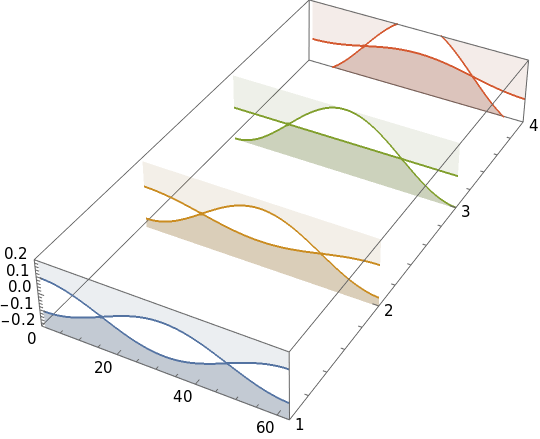
\includegraphics[width=0.7\textwidth]{figures/typeIIridgeline}
  \caption{\label{fig:ridgeline} \todo{Write this} }
\end{figure}
